\documentclass{beamer}
\usepackage{graphics}
\usepackage{beamerthemesplit}
\usetheme[hoptionsi]{Madrid}
%\usetheme{CambridgeUS}
\useinnertheme{rectangles}
%\usecolortheme{dolphin}
\logo{
\includegraphics[height=1.5cm]{logo.jpg}} %change here. I used an eps file logo, you can use jpg or other format
 \title[Technical Writing]{Technical Writing}
 \subtitle {How to Write Good Research Articles}
\author[Supta R. Philip] % (optional, use only with lots of authors)
{\textbf{Supta Richard Philip}~\inst{1}}
% - Give the names in the same order as the appear in the paper.
% - Use the \inst{?} command only if the authors have different
%   affiliation.
\institute[University of Trento] % (optional, but mostly needed)
{
  \inst{1}%
  M.Sc. in Computer Science\\
  Department of Information Engineering
and Computer Science\\
  University of Trento, Italy.}
 \date [\today]{\today \\ \ \\
 \tiny{ Copywrite Declaration : Metarials are taken from Dr. Ashfaqur Rahman, Research Scientist,Intelligent Sensing and Systems Lab (ISSL),CSIRO, Australia \& \\
Xiaohua Jia, Chair Professor,Dept of Computer Science,City University of Hong Kong.}
 
 }
 \begin{document}

 \frame{\titlepage}

 \section*{Outline}
 \frame{
\frametitle {Outline}
\tableofcontents}

\section{Publication Requirement}
 \frame
 {
 \frametitle {Publication Requirement}
The people who need the publications
 \begin{itemize}
 \item<1->  BSc Degree (Minor)
 \item<2-> MPhil Degree / MS by Research / MS (Minor)
 \item<3-> PhD Degree
 \item<4-> Full time researcher / Academics
 
 \end{itemize}
 }
 
  \section{Kinds of Scientific Publications}
 \frame
 {
 \frametitle {Kinds of Scientific Publications}

 \begin{itemize}
 \item<1-> Thesis \\
 Aspects to be Assessed for a Thesis:
 
  \begin{itemize}
 \item<5->  background knowledge
 \item<6-> 	original contributions (amount of work)
 \item<7-> 	methodology
 \item<8-> presentation (writing)
  \end{itemize}
	
 \item<2-> Conference Publications \\
 Focus on a piece of work with limited discussion

 \item<3-> Journal Publications \\
 More complete (extensive) discussion
 \item<4-> Book chapters / Text books

 \end{itemize}
 
 }



 \section{Where to publish your work}
 \frame
 {
 \frametitle {Where to publish your work}

 \begin{itemize}
 \item<1-> Journals\\ Ranking of journals \\
	Review process of journals \\
	Publication cycle
 \item<2-> Conferences \\
 Ranking of conferences \\
	Review process of conferences \\
N.B. a good journal / conference tends to have rigorous review process and long review time

 \end{itemize}
 
 }
 
 
   \subsection{ Important journals \& conferences}
 \frame
 {
 \frametitle { Important journals \& conferences}
\begin{itemize}
 \item<1-> Database \\
	IEEE Trans on Knowledge and Data Engineering\\
	ACM Trans on Database Systems\\
	Int�l Conf on VLDB 	
 \item<2-> Software Engineering \\
	IEEE Trans on Software Engineering\\
	ACM Trans on Software Eng. and Methodology\\
	IEEE Int�l Conf on Software Engineering
 \item<3-> Distributed Systems \\
	IEEE Trans on Parallel and Distributed Systems\\
	ACM Trans on Computer Systems\\
	IEEE Int�l Conf on Distributed Computing Systems
	 \item<4-> Computer Networks\\
	IEEE/ACM Trans on Networking\\
	IEEE INFOCOM\\
	ACM Mobicom, etc. 
	
	\end{itemize}


 }

 
 
 
 \section{Plan your writing}
 %\subsection{Overview of Smart Campus Project}
 \frame
 {
 \frametitle {Plan your writing}

 \begin{itemize}
 \item<1->  Ask two questions before starting:\\
	What is new in your work?\\
	What are you going to write?
 \item<2-> Emphasize on the originality and significance of your work.
 \item<3-> Organize your thinking and decide the structure (outlines) of your paper.
 \item<4-> Stick on your central points throughout the whole paper and remove all unnecessary discussions.

 \end{itemize}
 
 }
 \subsection{Reader-oriented Writing}
\frame{

 \frametitle {Reader-oriented Writing}
 
  \begin{itemize}
 \item<1->   Purpose of your writing: disseminating your research results.\\
	Don�t write if there is nothing to write.\\
	Don�t make a simple problem complicated to fool people.\\
	Don�t hide technical details.
	
	\item<2-> Reader-oriented writing: Write in a way that would lead readers to follow your thinking, NOT in the way of your thinking. \\
	Well-organize your thinking.\\
	Give enough and clear explanation (never leave reader to guess).\\
	Try to present your idea in an accurate way (no ambiguous).\\
	Always think how readers would interpret your writing (assume you�re a reader).
	
 \item<3->Use simple/ plain English.\\
	Purpose of technical writing: express your idea correctly \& clearly.
 \end{itemize}

}




 \section{Structure of a Paper}
 %\subsection{Contains}
  \frame
 {
 \frametitle {Structure of a Paper}

 \begin{itemize}
 \item<1-> Title
 \item<2-> Abstract
 \item<3-> Key words
 \item<4-> Introduction
 \item<5-> Background
 \item<6-> Related Work
 \item<7-> System Model \& Problem Statement
 \item<8-> Methods / Solutions
 \item<9-> Simulations / Experiments
 \item<10-> Conclusion
 \item<11-> Acknowledgement
 \item<12-> References
 \end{itemize}
\uncover<13->{Average number of pages of a journal paper.\\
Average number of pages of a conference paper.}

 }
 
%\section{Structure of a Paper}
\subsection{Choose a Right Title}
  \frame
 {
 \frametitle {Choose a Right Title}

 \begin{itemize}
 \item<1-> The title should be very specific, not too broad.
 \item<2-> The title should be substantially different from others.\\
 �Topology control for multihop wireless networks�, IEEE Trans. on Comm, 93.\\
�Topology control of multihop wireless networks using transmit power adjustment�, infocom�00.\\
�Distributed topology control for power efficient operation in multihop wireless networks�, infocom�01.\\
 \item<3-> Avoid general / big titles, e.g.,\\
 �Research on data mining�,\\
�Some research on job assignment in cluster computing�,\\
�A new framework for distributed computing�, 
 \end{itemize}
 }

%\section{Structure of a Paper}
\subsection{Write a concise Abstract}
  \frame
 {
 \frametitle {Write a concise Abstract}

 \begin{itemize}
 \item<1-> The use of an abstract:\\
 	for search purpose.\\
	giving readers a paper-summary before getting into details. 
 \item<2-> An abstract should tell:\\
the problem that the paper discusses.\\
the work that has been done, or method being used.\\
original findings / achievements. 
\item<3-> An abstract usually does NOT have:\\
reference numbers\\
multiple paragraphs
 \end{itemize}
 }
 
%\section{Structure of a Paper}
\subsection{Choose a right set of keywords}
  \frame
 {
 \frametitle {Choose a right set of keywords}

 \begin{itemize}
 \item<1-> The use of keywords:\\
 	database search,\\
	categorizing your work (for editors to choose reviewers).
 \item<2-> The keywords must be specific and, as a whole, represent the main topic of the paper.
\item<3-> Avoid using the words that are not the main topic, such as �calculus�, �simulations�, etc.

 \end{itemize}
 }
 
 \subsection{Examples of an abstract / keywords}
  \frame
 {
 \frametitle {Examples of an abstract / keywords}


\includegraphics[height=8cm,width=6cm]{abstract1.png} 
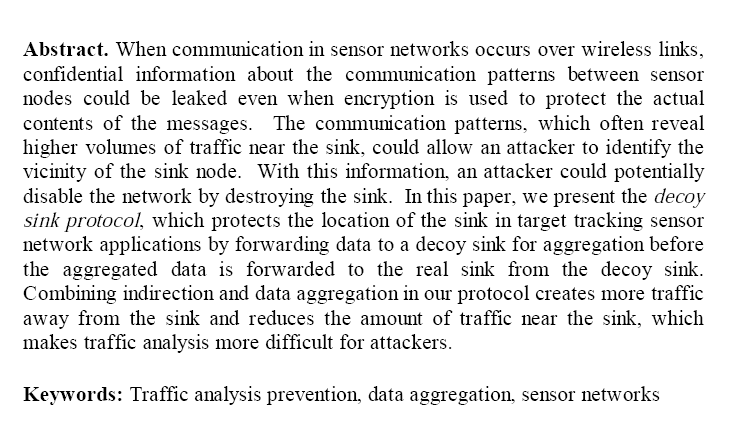
\includegraphics[height=8cm,width=6cm]{abstract.png} 
 } 
 
 \subsection{Organization of your Paper}
  \frame
 {
 \frametitle {Organization of your Paper}
 
 \begin{itemize}
 \item<1-> Top-down writing method
 \item<2-> Planning sections and subsections
 \item<3-> Sketching: use a sentence to represent the points (paragraphs) in each subsections
 \item<4-> Writing details: expand a sentence in the sketch into a paragraph
 \item<5-> Adjustment: break / merge paragraphs, add / merge sections
 \end{itemize}
\uncover<6->{N.B. keep a logical flow from section to section, paragraph to paragraph, and sentence to sentence.}

 }


 \subsection{Introduction: the most difficult part}
  \frame
 {
 \frametitle {Introduction: the most difficult part}
Purpose of introduction: 
	Introducing readers to your problem / work.
An introduction usually contains:
Brief background of the topic-area
Existing work, which would lead to the importance / originality of your work
Description of your problem
Achievement / significance / brief-methodology of work

}

 \subsection{Related work and Reference list}
  \frame
 {
 \frametitle {Related work and Reference list}
 
  %\begin{block}{ Proper selection of references:}
 \begin{itemize}
 \item<1->  Show your knowledge in the related area,
 \item<2-> Give credit to other researchers (reviewers are usually chosen from the references),
 \item<3-> Cite good quality work (particularly when citing your own work) and up to date work.
 \end{itemize}
 %\end{block}
 }
 % \subsection{Related work and Reference list}
  \frame
 {
 \frametitle {Related work and Reference list}

 % \begin{block}{ Related work should:}
 \begin{itemize}
 \item<1->  Be organized to serve your topic,
 \item<2-> Emphasize on the significance / originality of your work (Introducing your work out).
 \end{itemize}
 %\end{block}
 }
 % \subsection{Related work and Reference list}
  \frame
 {
 \frametitle {Related work and Reference list}
 
  %\begin{block}{Format of references:}
 \begin{itemize}
 \item<1->  Consistent with the format, ordering, etc.
 \item<2-> Standard format of books / journal papers / conference papers, e.g,\\
	X. Jia, X.D. Hu and D.Z. Du, Multiwavelength Optical Networks, Kluwer Academic, 2002.
	J. Li, Yi Pan, and X. Jia, �Analysis of Dynamic Location Management for PCS Networks�, IEEE Trans on Vehicular Technology, Vol. 51, No. 5, Sep 2002, pp.1109-1119.\\
	X. Jia, D. Li, X.Hu and D. Du, \"Placement of Read-Write Web Proxies in the Internet\", Proc of IEEE Int�l. Conf. on Distributed Computing Systems, Phoenix, USA, Apr 2001, pp.687-690.
 \item<2-> Do NOT use non-standard abbrev.
 \end{itemize}
 %\end{block}

}

 \subsection{Examples of reference lists}
  \frame
 {
 \frametitle {Examples of reference lists}
 
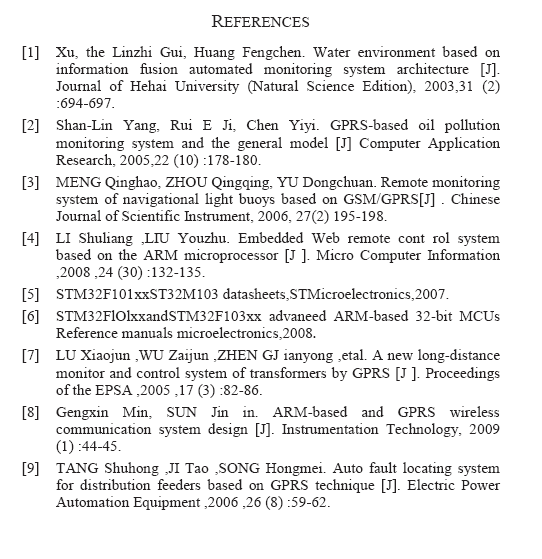
\includegraphics[height=8cm,width=6cm]{references.png} 
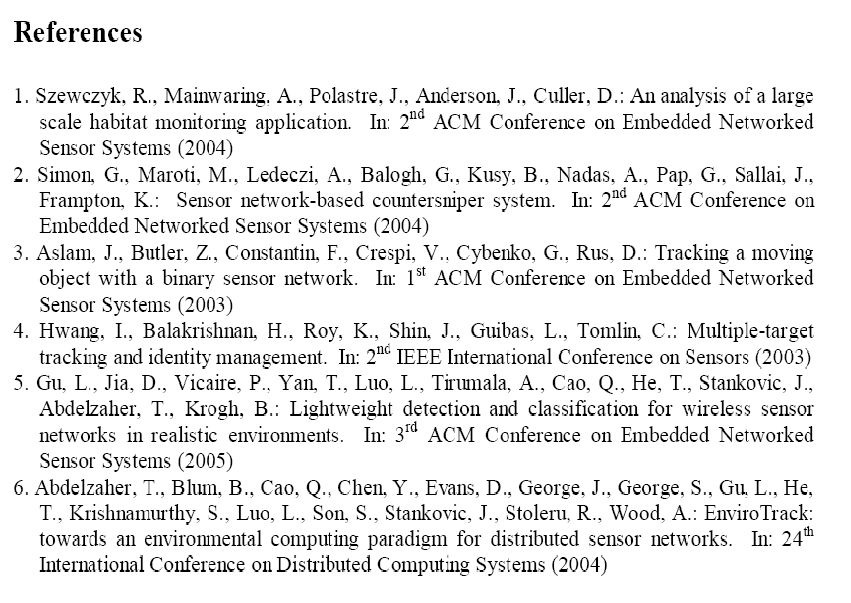
\includegraphics[height=8cm,width=6cm]{references2.png} 
 
 }
 
  \section{Writing Tips: carry you to a long way}
  \frame
 {
 \frametitle {Writing Tips: carry you to a long way}
 
 %\begin{block}{Writing Tips}
  \begin{itemize}
 \item<1->  Reader-oriented writing (good organization, logical flow, etc).

 \item<2-> Standard and consistent formatting (professional and neat looking).

 \item<3-> Learning from other people�s writing.

 \end{itemize}
 %\end{block}
 
 }
 
 
 % All of the following is optional and typically not needed. 
\appendix
\section<presentation>*{\appendixname}
\subsection<presentation>*{For Further Reading}

\begin{frame}[allowframebreaks]
  \frametitle<presentation>{For Further Reading}
    
  \begin{thebibliography}{10}
    
  \beamertemplatebookbibitems
  % Start with overview books.
  \bibitem{James}
   ~James D. Lester.
    \newblock {\em Writing Research Papers: A Complete Guide}.
    \newblock  Harpercollins College Div; 8th edition, January 1996.
 
     \bibitem{Peter}
   ~Peter Haisler.
    \newblock {\em Writing Research Papers: A Complete Guide}.
    \newblock  15/6 2011.

    
  \beamertemplatearticlebibitems
  % Followed by interesting articles. Keep the list short. 

  \bibitem{Sloman}
    A.~Sloman.
    %\newblock On this and that.
    \newblock {http://www.cs.bham.ac.uk/internal/research\_students/theses.php},
    Jul 2010.
  
    \bibitem{OCLC}
   ~OCLC Online Computer Library Center, Inc.
    %\newblock On this and that.
    \newblock http://www.aresearchguide.com/
  \end{thebibliography}

\end{frame}
 
 %\subsection{Examples of reference lists}
  % \frame
  %{
  %\frametitle {Examples of reference lists}


 %\begin{thebibliography}{[1]}
 %\bibitem{book:Lamport}
 %  Leslie Lamport, \textsl{\LaTeX: A Document Preparation}
  %System (2nd ed.), Addison-Wesley Publishing Company,
 %1994, ISBN 0-201-52983-1.
 %\bibitem{book:Goossens1}
 %Michel Goossens, Frank Mittelbach and Alexander Samarin,
 %\textsl{The \LaTeX{} Companion}, Addison-Wesley
 %Publishing Company, 1994, ISBN 0-201-54199-8.
 %\end{thebibliography}

  %}
 
\end{document}